\chapter{Results \& discussion}
\label{ch:Results discussion}
\begin{figure}
  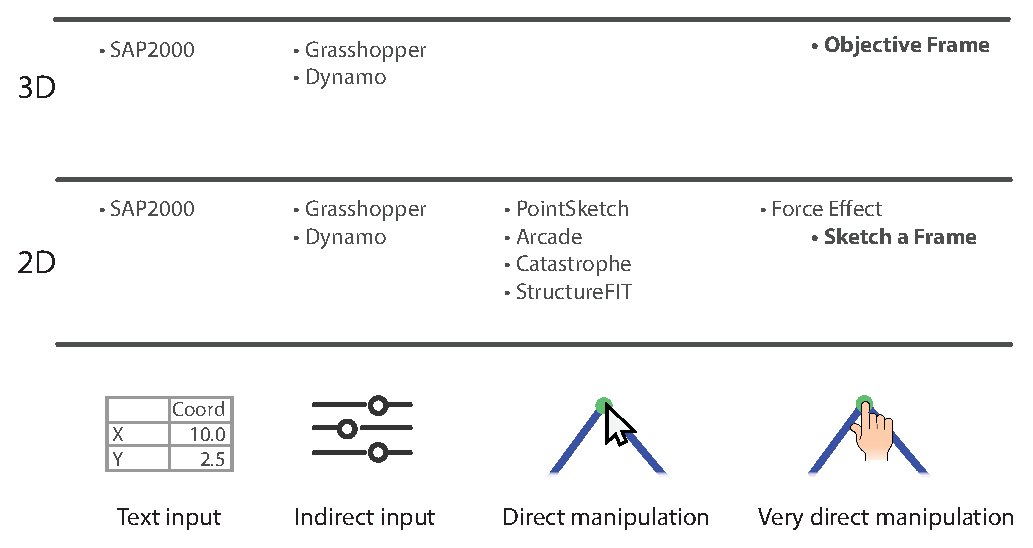
\includegraphics[width=330pt]{graphics/softwareReview.eps}
  \caption{Previous and work summarized in present work in bold}
  \label{fig:softwareReview}
\end{figure}

A summary of the evaluated conceptual design tools can be seen in Figure \ref{fig:softwareReview}, the tools are grouped according to number of dimensions and how direct the manipulation is experienced. The two developed applications have a higher degree of direct manipulation for 2D and for 3D than any other existing software for conceptual design. This is achieved by using novel technology, the multi-touch user interface for 2D and the Leap Motion Controller for 3D.

The thesis responds to a need for new, more intuitive and natural interaction modes in computational design and analysis. Very direct manipulation improves significantly beyond existing direct manipulation paradigms prevalent in computer-aided design. New technologies like the Leap Motion controller and the multi-touch interface open up unprecedented possibilities for engaging users in the exploration and design of structures. Which can improve the user’s understanding of the structural behavior of a model, cognitive engagement in the task performed, and encourage further design exploration.


\section{Summary of intellectual contributions}
\begin{itemize} 
\item Thesis includes critical review of existing tools and techniques for design manipulation in conceptual computer-aided design.
\item Paper A proposes a new direct manipulation cycle that automatically computes and presents the result when a structure is stable.
\item Paper A introduces new multi-touch interaction models for conceptual structural design on tablets.
\item Paper B is the first paper to propose very direct manipulation as human-computer interaction mode for 3D structures, thanks to new 3D input device such as Leap Motion controller
\item Paper B, introduces implemented design tool that allows users to interact with 3D structures through very direct manipulation.
\item Paper B demonstrates potential applications of 3D input devices through three case studies.
\end{itemize} 


\section{Future work}
The Leap Motion controller’s SDK supports virtual reality glasses, such as the Oculus Rift. Combining the two can create a virtual reality where the user can experience the structure in 3D, interact, and make changes to it using the hands. 

This could potentially be developed in a game environment where the structure could be visualized in the intended context i.e. the building site, a game engine would enable real-time renderings of the structure in its context. The designer would then be able to make manipulations, guided with performance feedback, to the rendered structure. 

Other existing design methods could be combined with this design environment, such as interactive optimization with the use of genetic algorithm. To improve computational speed, and allow fast generation of new designs, the design space can be approximated with the help of neural networks, also known as surrogate modeling. This can allow for more advanced structural models to be used for interactive optimization.

Case studies will be performed to study, and verify, the benefits of using the developed conceptual structural design tools. 